\section{Model predictive control}

Model predictive control (MPC) is an advance control method that depends on a dynamic model of the plant. MPC allows to calculate an optimal control signal taking the future electrical pricing into account. The control structure of MPC is in general 

\begin{figure}[H]
\centering
\begin{tikzpicture} [scale=0.67,transform shape]

\draw  (4.5,1.5) rectangle (7,-0.5);
%\node at (5.7,0.25) {Controller};
\node at (5.7,0.50) {System};

\draw  (-2,0) rectangle (0,-1);
\node at (-1,-0.5) {Model};

\draw  (-2,2) rectangle (0,1);
\node at (-1,1.5) {Optimizer};

\draw[dashed] (-5,4.5) rectangle (3,-1.5);

\draw[dashed]  (-4.5,3.5) rectangle (-2.5,2.5);
\node at (-3.5,3) {Obj-function};

\draw[dashed]  (0.5,3.5) rectangle (2.5,2.5);
\node at (1.5,3) {Constraints};

\draw[-triangle 60] (-4.25,0.75)-- (-4.25,1.5) -- (-2,1.5);
\draw[-triangle 60] (0.5,3)-- (-0.5,3) -- (-0.5,2);

\draw[-triangle 60] (2,0.5) -- (4.5,0.5);
\draw[-triangle 60] (7,0.5) -- (9.5,0.5);

\draw[-triangle 60] (-2.5,3)-- (-1.5,3) -- (-1.5,2);
%\draw[-triangle 60] (-5.5,0.5) -- (-4.5,0.5);

\draw[-triangle 60] (0,1.5) -- (2,1.5) -- (2,-0.5) -- (0,-0.5);
\draw[-triangle 60] (8,0.5) -- (8,-2) -- (-1,-2) -- (-1,-1);

\draw[-] (-2,-0.5) -- (-4.25,-0.5) -- (-4.25,0.75);

%\node at (-5.5,1) {$CP_{ref}$};
\node at (8.5,1) {$\bm{y}$};
\node at (0.5,2) {$\bm{u}_{Hp}$};
\node at (-2.5,0) {$\bm{y}_{Hp}$};
%\node at (-2.5,2) {$\widetilde{e}$};
\node at (3.7762,1) {$\bm{u}_{Hp}[k|k]$};
\node at (-1,4) {\textbf{MPC}};

%\draw  (-4.25,0.5) ellipse (0.25 and 0.25);
\draw[fill]  (2,0.5) ellipse (0.1 and 0.1);
\end{tikzpicture}%
 
\caption{The structure of the control with the MPC part specified \cite{Camacho2007}.}
\end{figure}

A MPC is a iterative process that can be setup as follows: 

\begin{itemize}
\item[1:] A model predict the future outputs, $\pmb{\tilde Y^*}$.
\item[2:] The outputs are compared to references, $CP_{ref}$.
\item[3:] The errors are feed back to the optimizer that calculate the future inputs $\tilde u$.
\item[4:] $u(k|k)$ is sent as the control signal for time k.
\item[5:] $\tilde u$ are applied to the model, together with the old outputs.
\item[6:] Go back to step 1 
\end{itemize}


%In this section the objective function, describing the electrical price, will be setup. Furthermore the MPC will be designed. 

\chapter{Electrical price}\label{sec:cost_fkt} %\todotom{I think it is a good idea to treat the data below as if it were a prediction of the future prices.
%W.r.t. the term 'cost function', I think it's a bit misplaced here. What you have in the graph is the cost-of-energy as a function of time. However, when you use the term 'cost function' it might be confused with the term 'objective function', which in your case will be the product between the cost-of-energy and the energy consumed.}
%
%
To minimize the running cost of the system, the power consumption of the pumps, $P_e$ Cf. \secref{PumpModel}, and the electrical price, $c_p[k]$, is considered. Predicting future prices is an extensive task that depends on many factors e.g user consumption and weather conditions. Due to the fact that the main focus of this project is not to derive a high precision predictive model that describe future electrical prices, data is used from \cite{Electrical_price} instead. The price function can be seen in \figref{fig:electrical_price}. 


% Due to the fact that the learning goals of this project is not to derive a high precision predictive model that describe future electrical prices, a simple model that mimics real electrical pricing is created. This model is based on electrical pricing in Denmark from the period 27-03-2017 to 02-04-2017.  


% To predict future prices a simple moving average (SMA) is used.
% This approach have been chosen, .

% The SMA uses present and previous data samples to calculate future predictions, this can be expressed as seen in \eqref{equ:MA}.
	
% \begin{equation}
% x(k+1) = \frac{1}{N}\sum\limits_{k=0}^{N-1} x(-k)
% \label{equ:MA}
% \end{equation} 

% The SMA can not take non-stationary processes into account, so if sudden changes in the price appears, the future estimates will be less precise. From \cite{Electrical_price} data price over the present has been gathered and can be seen on \figref{fig:electrical_price} together with the SMA model which utilize the previous data sample and the present. 

\begin{figure}[H]
\centering
% This file was created by matlab2tikz.
%
%The latest updates can be retrieved from
%  http://www.mathworks.com/matlabcentral/fileexchange/22022-matlab2tikz-matlab2tikz
%where you can also make suggestions and rate matlab2tikz.
%
\definecolor{mycolor1}{rgb}{0.00000,0.44700,0.74100}%
\definecolor{mycolor2}{rgb}{0.85000,0.32500,0.09800}%
%
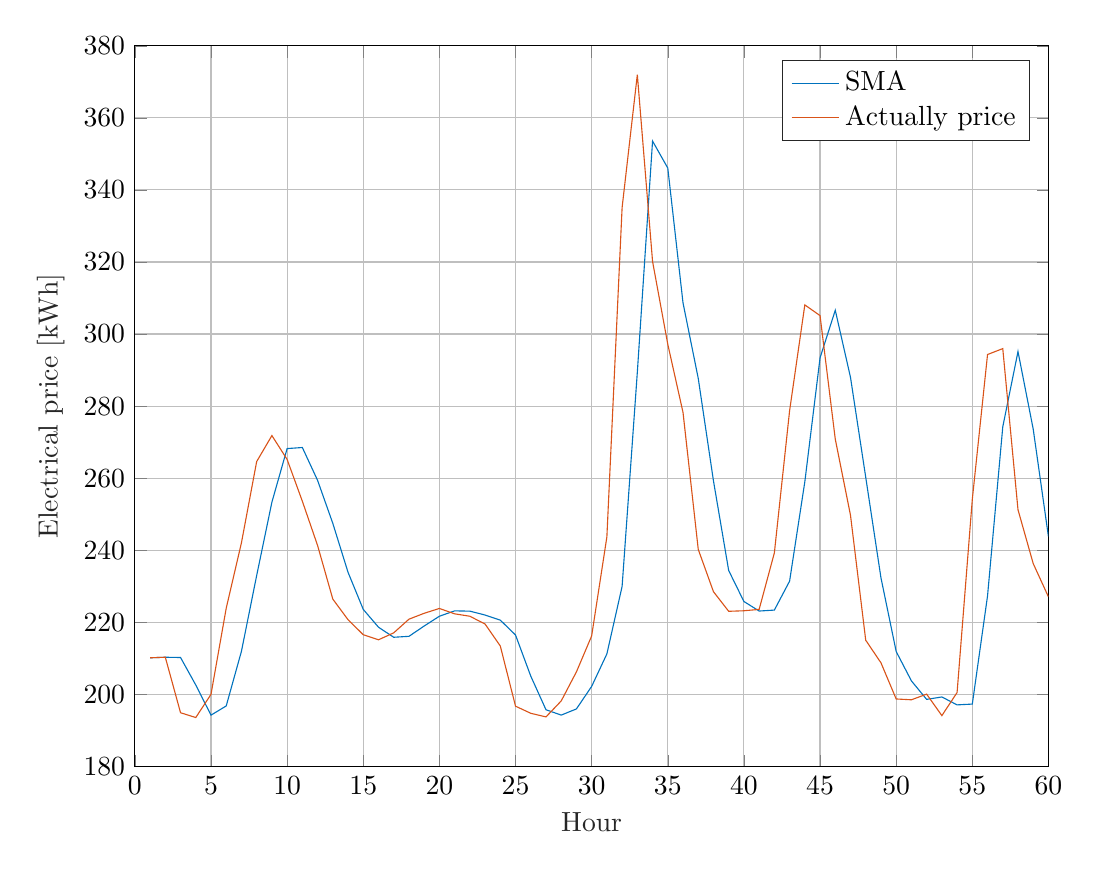
\begin{tikzpicture}

\begin{axis}[%
width=4.568in,
height=3.603in,
at={(0.766in,0.486in)},
scale only axis,
xmin=0,
xmax=60,
xlabel style={font=\color{white!15!black}},
xlabel={Hour},
ymin=180,
ymax=380,
ylabel style={font=\color{white!15!black}},
ylabel={Electrical price [kWh]},
axis background/.style={fill=white},
xmajorgrids,
ymajorgrids,
legend style={legend cell align=left, align=left, draw=white!15!black}
]
\addplot [color=mycolor1]
  table[row sep=crcr]{%
1	210.15\\
2	210.3\\
3	210.225\\
4	202.6\\
5	194.2325\\
6	196.7825\\
7	211.955\\
8	232.99\\
9	253.34\\
10	268.215\\
11	268.51\\
12	259.4\\
13	247.46\\
14	233.88\\
15	223.58\\
16	218.635\\
17	215.845\\
18	216.105\\
19	218.965\\
20	221.68\\
21	223.17\\
22	223.095\\
23	222.015\\
24	220.6\\
25	216.4725\\
26	205.0725\\
27	195.7325\\
28	194.2425\\
29	195.955\\
30	202.205\\
31	211.225\\
32	229.955\\
33	289.4\\
34	353.555\\
35	346.08\\
36	308.655\\
37	287.71\\
38	259.25\\
39	234.365\\
40	225.77\\
41	223.125\\
42	223.39\\
43	231.425\\
44	258.99\\
45	293.4\\
46	306.605\\
47	287.97\\
48	260.255\\
49	232.355\\
50	211.89\\
51	203.74\\
52	198.605\\
53	199.275\\
54	197.08\\
55	197.3\\
56	227.32\\
57	274.23\\
58	295.14\\
59	273.6\\
60	243.765\\
};
\addlegendentry{SMA}

\addplot [color=mycolor2]
  table[row sep=crcr]{%
1	210.15\\
2	210.3\\
3	194.9\\
4	193.565\\
5	200\\
6	223.91\\
7	242.07\\
8	264.61\\
9	271.82\\
10	265.2\\
11	253.6\\
12	241.32\\
13	226.44\\
14	220.72\\
15	216.55\\
16	215.14\\
17	217.07\\
18	220.86\\
19	222.5\\
20	223.84\\
21	222.35\\
22	221.68\\
23	219.52\\
24	213.425\\
25	196.72\\
26	194.745\\
27	193.74\\
28	198.17\\
29	206.24\\
30	216.21\\
31	243.7\\
32	335.1\\
33	372.01\\
34	320.15\\
35	297.16\\
36	278.26\\
37	240.24\\
38	228.49\\
39	223.05\\
40	223.2\\
41	223.58\\
42	239.27\\
43	278.71\\
44	308.09\\
45	305.12\\
46	270.82\\
47	249.69\\
48	215.02\\
49	208.76\\
50	198.72\\
51	198.49\\
52	200.06\\
53	194.1\\
54	200.5\\
55	254.14\\
56	294.32\\
57	295.96\\
58	251.24\\
59	236.29\\
60	227.06\\
};
\addlegendentry{Actually price}

\end{axis}
\end{tikzpicture}%
\caption{$c_p[k]$, describing the electricity prices in Denmark from the 27-03-2017 to 02-04-2017.}
\label{fig:electrical_price} 
\end{figure}

As this is a real data from a given period, most likely it does not fit the pricing in any other given week, as the pricing is fluctuating a lot from day to day. However, the data indicates that the pricing is higher in the morning and evening which is applicable for any given week and thereby is a general property of the time dependent pricing. This behavior can be seen as the periodicity of the data with two peaks a day. The chosen data thus gives a realistic idea of the improvement of the controller which can be achieved in a real world scenario based on the week on which the data is recorded.  

%However $\frac{1}{\eta}\cdot\Delta p \cdot q \cdot \Gamma(k)$ 

% Even though the pricing seen in \figref{fig:electrical_price} is not a prediction of the future electrical pricing it is assumed to be a good representation of the pricing and therefor it will be used for this project. 


\subsection{Constraints}

When designing a MPC the constraints have to be setup so they represent actuator slew rates, actuator ranges and constraints for the control variables. These constraints are setup as matrices called $\pmb{E}, \pmb{F} \text{and} \:\pmb{G}$. The constraints matrices are given by: 

\begin{equation}
\pmb{E} \cdot [\Delta\tilde u(k|k),...,\Delta\tilde u(k+H_u-1|k),1]^T \leq 0 
\label{eq:slewrate}
\end{equation}
\begin{equation}
\pmb{F} \cdot [\tilde u(k|k),...,\tilde u(k+H_u-1|k),1]^T \leq 0 
\label{eq:actranges}
\end{equation}
\begin{equation}
\pmb{G} \cdot [\tilde y(k+H_w|k),...,\tilde y(k+H_p|k),1]^T \leq 0
\label{eq:controlvar}
\end{equation}


 \begin{minipage}[t]{0.20\textwidth}
 Where\\
 \hspace*{8mm} $\tilde u(k|k)$ \\
 \hspace*{8mm} $\Delta\tilde u(k|k)$ \\
 \hspace*{8mm} $H_u$ \\
 \hspace*{8mm} $H_w$ \\
 and \hspace*{0.7mm} $\tilde y(k+H_w|k)$	
 \end{minipage}
 \begin{minipage}[t]{0.68\textwidth}
 \vspace*{2mm}
 is the input vector, \\
 is the change of the input vector, \\
 is the control horizon, \\
 is the window horizon, \\
 is the estimate of the controlled output to the time $k+H_w$ compared to current output.
 \end{minipage}

The actuator slew rate constraint, matrix $\pmb{E}$, determents how fast the actuator can change per time unit. From this the physical limit of the pumps can be described. The actuator ranges describe how the control signal to the pumps should look. This is simply a way to describe 0 to 100 \% performance. In the case of this project the pumps can be controlled with an input from 0 to 5. The constraints on the control variables is the constraints setup in \secref{control_problem}. \todo{This part could properly be specified better.}

%To easy notation $U(k) = $

%As it can be seen from \eqref{eq:slewrate,eq:actranges,eq:controlvar} depend on three different variables $\hat u(k|k), \Delta\hat u(k|k) \text{and} \hat z(k+H_w|k)$

To calculate the constraint matrices $H_p, H_u \text{and} \: H_w$ need to be determined. In \secref{sec:cost_fkt} the electrical price is described. From this it can be seen that the price fluctuates a lot but some periodicity can be seen every 24 hours. Therefor both $H_p$ and $ H_u $ are set to 24. 

\todoque{How sould we chose $H_w$}

% The plan from here on is: 

% 1: Describe the transformation of the constraints so they all depend on delta U(k) 

% 2: Explain how the minimization problem can be set up in general and then s.t. the new constrains 

% 3: Cover why we need an observer and what it means for how the minmization problem is set up - U(k) -> \hat U(k|k)
